\chapter{Аналитическая часть}

В данном разделе проводится анализ способов хранения и агрегирования данных, а также  систем управления базами данны. Определяется постановка задачи.

\section{Постановка задачи}

Разработать веб-сервис “Анализатор Олимпийских игр” для отображения количества 
призовых мест по задаваемым характеристикам 
(имя, возраст, пол, вес, рост спортсмена, а также страна, вида спорта и дисциплина вида спорта).

Предусмотреть роли: авторизованный пользователь, не авторизованный пользователь и администратор. Реализовать создание аккаунта и добавление комментариев.
Для роли администратора реализовать удаление комментариев и пользователей. Для роли неаутентифицированны пользователь запретить использование сервиса и добавление комментариев.

\newpage
\section{Формализация данных}

В базе данных должна храниться информация о следующих моделях:

\begin{itemize}
	
	\item Атлеты;
	
	\item Олимпиады;
	
	\item Страны;
	
	\item Результаты;
	
	\item Виды спорта;
	
	\item Дисциплины вида спорта;
	
	\item Таблица пользователей;
	
	\item Комментарии;
	
	\item Буфер комментариев;
	
\end{itemize}

Иформация о категориях и данных приведены в таблице \ref{tab:category}


\newpage
\begin{table}[h!]
\caption{Категории и сведения о данных}
\label{tab:category}
	\begin{tabular}{ | p{100pt} | p{350pt}  | }
		\hline
		Категория & Сведения   \\ \hline
		
		Атлеты & Имя, пол, возраст, вес, рост, \\
	 	            & идентификатор страны, идентификатор вида спорта  \\
					&   \\ \hline
		Страны & Код страны, название страны, столица, население  \\
					 &   \\ \hline 
		
		
		Олимпиады & Город проведения, год проведения, \\
		                    & сезон года(лето, осень)   \\
		                    &   \\ \hline
		
		Результаты & Идентификатор спортсмена,  \\
		                   &  идентификатор Олимпиады, \\
		                   & идентификатор вида спорта, \\
		                   & идентификатор дисциплины вида спорта, \\
		                   & проверка золотой медали, \\
		                   & проверка серебренной медали, \\
		                   & проверка бронзовой медали \\
		                   &   \\ \hline 
		
		Виды спорта & Название вида спорта  \\
		                     &   \\ \hline 
		                     
		Дисциплины вида спорта & Идентификатор вида спорта, название дисциплины  \\
		&   \\ \hline 
		
		Таблица пользователей & Имя аккаунта, почта пользователя, проверка на админа, пароль, роль пользователя, дата, время регистрации, имя, фамилия, проверка активности пользователя.  \\
		&   \\ \hline   
		
		Комментарии & Идентификатор пользователя, текст, дата публикации, время публикации  \\
		&   \\ \hline 
		
		Буффер комментариев & Идентификатор пользователя, текст, дата публикации, время публикации  \\
		&   \\ \hline 
		 
	\end{tabular}
\end{table}

\newpage
\section{Типы пользователей}

Для доступа к основным функциям веб-сервиса, необходимо предусмотреть ролевую модель \cite{role-m}.
Для управления действиями пользователей принято решение ввести три роли: гость(неавторизованный пользователь), авторизованный пользователь и администратор.


Информация о типах пользователей и их возможностях представлены в таблице \ref{tab:users}

\begin{table}[h!]
	\caption{Типы пользователей и их возможности}
	\label{tab:users}
	\begin{tabular}{ | p{150pt} | p{300pt}  | }
		\hline
	    Тип пользователя & Возможности   \\
	     \hline
		
		Гость & Доступ к просмотру комментариев и авторизации \\
		&   \\ \hline
		
		Авторизованный пользователь & Доступ к главной странице, возможности произвести поиск, просмотр и добавление комментариев, возможность выйти из системы  \\
		&   \\ \hline 
		
		
		Администратор & Доступ к главной странице, возможности произвести поиск, просмотр, добавление и удаление комментариев, возможность выйти из системы, удаление пользователей. \\
		&   \\ \hline
		
		
	\end{tabular}
\end{table}

\newpage

\section{Базы данных и системы управления базами данных}

Для анализа и агригирования данных важную роль играет модель хранения данных,
которая будет использоваться для хранения информации о спортсменах, 
результатов, стран, видов спорта, пользователей и комментариев.

Для хранения данных используются базы данных \cite{database}. Для управления базами данных используются 
системы управления базами данных (сокращенно СУБД) \cite{subd}. Система управления базами данных — 
это совокупность программных и лингвистических средств общего или специального назначения, 
обеспечивающих управление созданием и использованием баз данных.

\section{Хранение данных о пользователях и Олимпийских играх}

Разрабатываемый в рамках курсового проекта сервис предполагает собой два приложения:

\begin{enumerate} 
	\item Для анализа и агрегирования данных
	
	\item Для отображения результатов, полученных первым приложением, а также обработки действий пользователей в графическом интерфейсе
	
\end{enumerate}

Каждое из двух приложений имеет права, отличные от другого. 
Первое должно иметь возможность читать данные, отвечающие за информацию о спортсменах 
и их результатах, второе же должно иметь возможность читать, записывать и удалалять 
данные пользователей и комментарии.

\newpage

Для хранения информации о Олимпийских играх необходимо использовать строго типизированную 
базу данных, т.к. все данные имеют четко выраженную структуру, неподдающуюся изменениям.

\section{Классификация баз данных по способу хранения}

Способы хранения баз данных  бывают двух видов: колоночные и строковые. 
Каждый из этих видов хранения подходит для реализации определенных задач.


\subsection{Колоночные базы данных}

Записи в базах данных колоночного типа представляются по столбцам (в памяти). Данный тип используется в аналитических система, которые характеризуется низким объемом транзакций, а запросы часто сложны и включают в себя агрегацию. Показателем эффективности системы является время отклика.

\subsection{Строковые базы данных}

Записи в базах данных строкового типа представляются построчно (в памяти). 
Для таких систем характерно большое количество коротких транзакций с операциями вставки, 
обновления и удаления данных. Зачастую их используют в транзакционных системах.
Основными задачами транзакционных систем являются: поддержание целостности данных, быстрая обработка запросов. Показателем эффективности системы является количество транзакций в секунду.

\section{Способы агрегации данных}

Для сбора информации о результатах, зависящих от задаваемых характеристик, необходима агрегация данных.

\subsection{Встроенные агрегатные функции базы данных}

Современные базы данных содержат в себе механизмы анализа -- \\ 
агрегатные функции (агрегаторы) \cite{agr-f}.
Агрегатные функции получают \\ единственный результат из набора входных значений. 

Значения нескольких строк или столбцов группируются вместе, образуя единое итоговое значение.

Примеры агрегатных функций:
\begin{itemize}
	\item Нахождение среднего
	
	\item Нахождение среднего
	
	\item Подсчёт количества
	
	\item Нахождение максимума
	
	\item Нахождение минимума
	
	\item Нахождение суммы
	
	\item и другие
\end{itemize}

\newpage

\subsection{OLAP}

OLAP (Online analytical processing) \cite{olap} -- это технология обработки данных для выполнения 
многомерного анализа на высокой скорости больших объемов данных из хранилища данных.

Большое количество данных имее несколько измерений - несколько категорий, по которым можно разбить информацию для более детального представления или анализа. 
Например, показатели продаж могут иметь несколько измерений, связанных с местоположением (регион, страна,  магазин), временем (год, месяц, неделя, день, часб секунды), продуктом (одежда,  мужчины/женщины/дети, бренд), и другие.

В хранилище данных наборы данных хранятся в таблицах, каждая из которых может упорядочивать данные только по двум из этих измерений одновременно. OLAP извлекает данные из нескольких наборов реляционных данных и реорганизует их в многомерный формат, который обеспечивает очень быструю обработку и очень глубокий анализ.

Фактически, OLAP-сервер обычно является средним аналитическим уровнем решения для хранилища данных.


\subsection*{OLAP Сube}

 OLAP Сube или MOLAP (Multidimensional OLAP) \cite{olap-cube} -- это многомерная база данных на основе массивов, которая позволяет обрабатывать и анализировать несколько измерений данных намного быстрее и эффективнее, чем традиционная реляционная база данных .
 
 Таблица реляционной базы данных структурирована как обычная таблица, в которой отдельные записи хранятся в двухмерном формате по строкам и столбцам. Каждый «факт» в базе данных находится на пересечении двух измерений - строки и столбца.
 
 Инструменты отчетов SQL и реляционных баз данных, безусловно, могут запрашивать и анализировать многомерные данные, хранящиеся в таблицах, но производительность снижается по мере увеличения объемов данных.
 
 Многомерная база данных создаётся путём расширения реляционной базы данных дополнительными слоями и измерениями (осями), состоящими из уровней.
 Например, верхний слой куба может упорядочивать продажи по местам, а подслоями могут быть страна, город, пункт выдачи. 
 После расширения системы хранения данных куб полностью собирается и сохраняется в памяти машины.
 
 Теоретически куб может содержать бесконечное количество слоев, но на практике аналитики данных создают OLAP кубы, содержащие только те слои, которые им нужны, для оптимального анализа и производительности.
 
 Одними из примуществ OLAP куба является то, что нет необходимости хранить реляционную базу данных из которой сформирован куб, т.к. после сборки он сохраняется обособленно от системы хранения данных и не зависит от её типа (строкового или колоночного). Из этого вытекает главный минус: необходима дополнительная память для хранения куба.
 
 OLAP кубы позволяют выполнять четыре основных типа операций многомерного анализа данных:
 
\begin{itemize}
 	\item Детализация (Drill-down)
 	
 	\item Свертывание (Roll up)
 	
 	\item Срез (Slice and dice)
 	
 	\item Поворот (Pivot)
 	
\end{itemize}

\newpage

На рисунке \ref{fig:cube-example} изображён пример представления  OLAP куба, содержащего 3 оси: время, продукт, место.\\


\begin{figure}[!h]
	\center{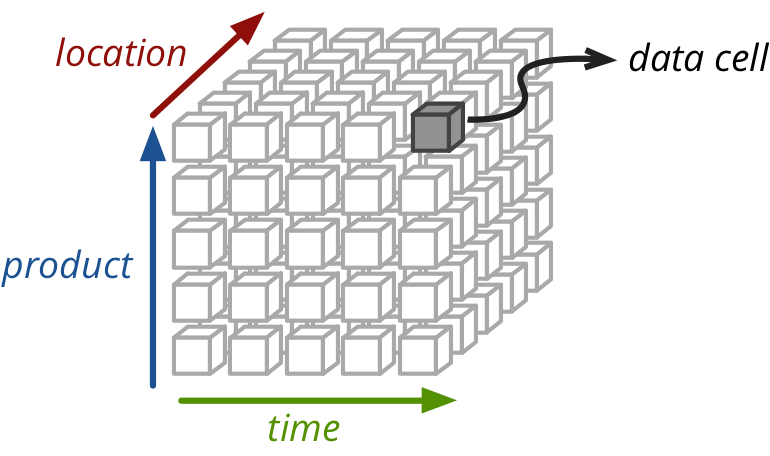
\includegraphics[scale=0.8]{img/cubes-example.png}}
	\caption{Пример трёхмерного OLAP куба}
	\label{fig:cube-example}
\end{figure}

На рисунке \ref{fig:cubes-operations} изображён пример представления 4х основных операций над OLAP кубом.

\begin{figure}[!h]
	\center{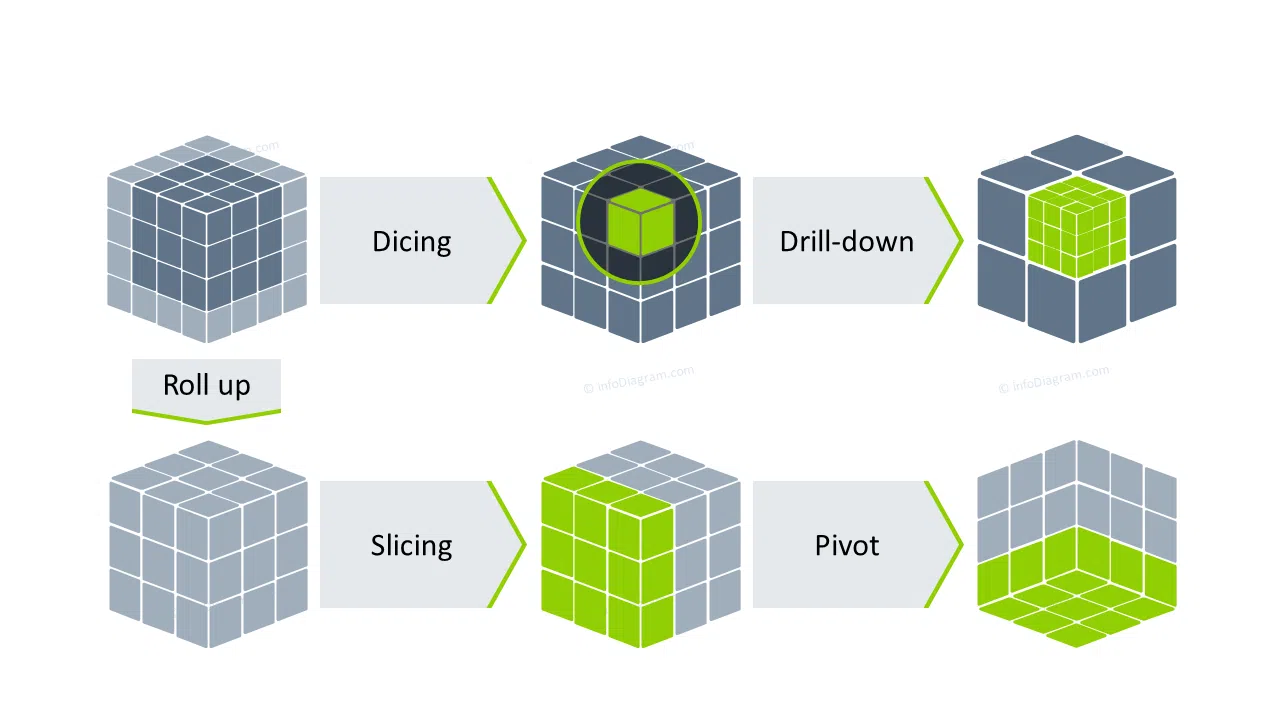
\includegraphics[scale=0.35]{img/cubes-operations.png}}
	\caption{Пример операций над OLAP кубом}
	\label{fig:cubes-operations}
\end{figure}

\subsection*{ROLAP}

ROLAP (Relational OLAP) \cite{olap} -- это многомерный анализ данных, который работает непосредственно 
с данными в реляционных таблицах, без предварительной реорганизации данных в куб.

Как отмечалось ранее, SQL - это превосходный инструмент для многомерных запросов, отчетов и анализа. Но требуемые SQL запросы сложны, производительность может замедляться, а результирующее представление данных является статическим - его нельзя преобразовать для отображения другого представления данных. ROLAP лучше всего подходит, когда возможность работать с большими объемами данных напрямую важнее, чем производительности и гибкости.


\subsection*{HOLAP}

При использовании HOLAP (Hybrid OLAP) \cite{olap} происходит пытака создать оптимальное разделение труда между 
реляционными и многомерными базами данных в рамках единой архитектуры OLAP.
Реляционные таблицы содержат большие объемы данных, а кубы OLAP используются для агрегирования и спекулятивной обработки. 
Для HOLAP требуется сервер OLAP, поддерживающий как MOLAP, так и ROLAP.

Инструмент HOLAP может «детализировать» куб данных до реляционных таблиц, что открывает путь для быстрой обработки данных и гибкого доступа. 
Эта гибридная система может предложить лучшую масштабируемость, но не может избежать неизбежного замедления при доступе к реляционным источникам данных. 
Кроме того, его сложная архитектура обычно требует более частых обновлений и обслуживания,
поскольку она должна хранить и обрабатывать все данные из реляционных баз данных и многомерных баз данных. 
По этой причине HOLAP может оказаться более долгим и требовательным.


\section{Выбор способа агрегации данных для решения задачи}

Для решения задачи был выбран способ создания OLAP Cube (MOLAP),
 т.к. он выигрывает в скорости у обычной реалиционной базы данных, 
 после его сборки не требуется дополнительное вмешательсто со стороны пользователя, 
 а также есть возможность размещения на сервер, в качестве отдельного приложения.
 
 
\section{Выбор модели хранения данных для решения задачи}

Для решения задачи было выбрано построчное хранение данных по нескольким причинам:

\begin{itemize}
	\item Для реализации приложения анализа данных собирается OLAP Cube, 
	который не зависит от модели хранения данных, 
	а значит нет причин не использовать построчное хранение;
	
	\item Для приложения, отображающего полученные данные из первого \\(OLAP Cube)
	не предполагается выполнения аналитических запросов;
	
	\item Для второго приложения, предполагает постоянное добавление, изменение данных о коментариях и пользователях;
	
	
\end{itemize}

\subsection{Обзор СУБД с построчным хранением}
	
	В данном подразделе буду рассмотрены популярные построчные СУБД, которые могут быть использованы для реализации хранения в разрабатываемом программном продукте.
	

\subsection*{PostgreSQL}

PostgreSQL \cite{postgresql} – это свободно распространяемая объектно-реляционная система управления базами данных, наиболее развитая из открытых СУБД в мире и являющаяся реальной альтернативой коммерческим базам данных.

PostgreSQL предоставляет транзакции со свойствами атомарности, согласованности, изоляции, долговечности (ACID), автоматически обновляемые представления, материализованные представления, триггеры, внешние ключи и хранимые процедуры. Данная СУБД предназначена для обработки ряда рабочих нагрузок, от отдельных компьютеров до хранилищ данных или веб-сервисов с множеством одновременных пользователей.

Рассматриваемая СУБД управляет параллелизмом с помощью технологии управления многоверсионным параллелизмом (англ. MVCC). Эта технология дает каждой транзакции «снимок» текущего состояния базы данных, позволяя вносить изменения, не затрагивая другие транзакции. Это в значительной степени устраняет необходимость в блокировках чтения и гарантирует, что база данных поддерживает принципы ACID.

\subsection*{MySQL}
MySQL \cite{mysql} – свободная реляционная система управления базами данных. Разработку и поддержку MySQL осуществляет корпорация Oracle.

Рассматриваемая СУБД имеет два основных движка хранения данных: InnoDB и myISAM. Движок InnoDB полностью совместим с принципами ACID, в отличии от движка myISAM. СУБД MySQL подходит для использования при разработке веб-приложений.
Реализация параллелизма в СУБД MySQL реализовано с помощью механизма блокировок, который обеспечивает одновременный доступ к данным.


\subsection*{Oracle Database}
Oracle Database \cite{oracle} – объектно-реляционная система управления базами данных компании Oracle. На данный момент, рассматриваемая СУБД является самой популярной в мире.

Все транзакции Oracle Database соответствуют свойствами ACID, поддерживает триггеры, внешние ключи и хранимые процедуры. Данная СУБД подходит для разнообразных рабочих нагрузок и может использоваться практически в любых задачах. Особенностью Oracle Database является быстрая работа с большими массивами данных.

Oracle Database может использовать один или более методов параллелизма. Сюда входят механизмы блокировки для гарантии монопольного использования таблицы одной транзакцией, методы временных меток, которые разрешают сериализацию транзакций и планирование транзакций на основе проверки достоверности.

\subsection{Выбор СУБД для решения задачи}

Для решения задачи была выбрана СУБД PostgreSQL, потому что данная СУБД проста в развертывании, имеет документацию на русском языке, а также легко интегрируема в приложение, написанное на языке программирования python \cite{python} из-за большого числа библиотек для работы с ней.


\section*{Вывод}

В данном разделе:

\begin{itemize}
	
	\item Была проанализирована поставленная задача и описаны способы ее реализации.
	
	\item Был проведен анализ СУБД, и выбрана оптимальная СУБД для решения задачи;
	
	\item Был выбран наиболее подходящий способ анализа и агригирования данных;
	
\end{itemize}
	
 










